% =====================================================================
% Clase -- Física 11° -- Trimestre I -- Semana 05
% Sesiones 008 (lun 28 sep., 11:00, 100 min) y 009 (mié 30 sep., 10:10, 100 min)
% Temas 2 y 3 de la guía: La carga eléctrica; Ley de Coulomb · hilo «De Tales al pararrayos»
% Material del docente (no se entrega a los estudiantes).
% =====================================================================
\documentclass[11pt]{article}
\makeatletter\def\input@path{{../../../../../plantillas/estilo/}}\makeatother
\usepackage{mmcantillo}
\guiadelestudiante{../../guia-didactica/guia-periodo-I-electrostatica}

\tipodocumento{Clase}
\asignatura{Física}
\titulo{Semana 5: de la lista de materiales a la fórmula}
\grado{11°}
\periodo{I}

% DBA: naturales grado 11 · DBA 2 — Comprende la naturaleza de la carga eléctrica y las
% interacciones entre cuerpos cargados, y explica fenómenos electrostáticos y la ley de
% Coulomb. Evidencias de la semana: interpretar los resultados de un montaje experimental
% propio en términos de transferencia de carga (sesión 008) y usar la ley de Coulomb para
% predecir y calcular la fuerza entre cargas puntuales (sesión 009).

\begin{document}

\encabezado*

\begin{center}
{\renewcommand{\arraystretch}{1.3}
\begin{tabularx}{\linewidth}{@{}l l l X l@{}}
  \toprule
  \textbf{Sesión} & \textbf{Fecha} & \textbf{Min} & \textbf{Subtema} & \textbf{Entregables}\\
  \midrule
  008 & lun 28 sep., 11:00 & 100 & Puesta en común del laboratorio; Gilbert y el
        \emph{De Magnete} & Taller (5 pts)\\
  009 & mié 30 sep., 10:10 & 100 & Ley de Coulomb: enunciado, fórmula, constante y unidades
      & Quiz (5 pts)\\
  \bottomrule
\end{tabularx}}
\end{center}

La semana pasada el salón frotó, colgó y observó. Esta semana esos resultados se vuelven
conocimiento: primero poniéndolos en común y comparándolos con lo que hizo William Gilbert en
1600 —que es exactamente lo mismo, con los mismos materiales—, y después dándoles la forma
cuantitativa que les faltaba, la ley de Coulomb. Referencias:
\refguia{tema:carga} y \refguia{tema:coulomb}.

% ---------------------------------------------------------------------
\seccion{Sesión 008 — lunes 28 de septiembre · 11:00 · 100 min}

\textbf{Objetivo.} Ordenar los resultados del laboratorio en una sola serie triboeléctrica
acordada por el curso, explicar cada observación en términos de transferencia de electrones, y
reconocer en el trabajo de Gilbert el mismo método.

\textbf{Materiales.} Los cuadernos de laboratorio de la sesión 007; tablero; un tubo de PVC,
lana y un electroscopio a la mano para repetir lo que haga falta; la guía.

\begin{center}
{\renewcommand{\arraystretch}{1.3}
\begin{tabularx}{\linewidth}{@{}l l X@{}}
  \toprule
  \textbf{Momento} & \textbf{Min} & \textbf{Actividad}\\
  \midrule
  Tabla común & 0--25 & Cada grupo pasa al tablero y anota qué pasó con sus parejas de
    materiales. Se arma una sola tabla del curso. Casi con seguridad habrá resultados que no
    coinciden: \textbf{no se borran}. Se marcan y se pregunta qué pudo cambiar (humedad,
    material distinto del que dice el nombre, frotado corto). Es el momento más valioso de la
    sesión.\\
  La serie & 25--45 & Ordenar los materiales en una sola fila, del que más tiende a quedar
    positivo al que más tiende a quedar negativo, usando solo los resultados de la tabla.
    Comparar con la serie triboeléctrica de la guía. Discutir las diferencias con el mismo
    criterio de antes: ¿dato malo o condición distinta?\\
  Explicación & 45--62 & Releer tres resultados en el lenguaje correcto: no «se cargó», sino
    «pasaron electrones de A a B». Insistir en que la carga no se crea: lo que uno gana, el
    otro lo pierde, exactamente. El caso de la inducción (el PVC acerca sin tocar y el
    electroscopio reacciona) se explica aparte: ahí la carga total sigue siendo cero.\\
  Gilbert & 62--78 & 1600, \emph{De Magnete}. Gilbert probó decenas de materiales uno por uno,
    con un versorium —una aguja que gira sobre una punta— y llamó «eléctricos» a los que se
    comportaban como el ámbar. Fue quien separó el magnetismo de la electricidad, que hasta
    entonces se confundían. Punto del hilo: el salón acaba de hacer, en dos sesiones, lo que
    él hizo durante años; la diferencia no es el ingenio, es que él no tenía a quién
    preguntarle.\\
  Taller & 78--95 & Taller de la sesión (5 puntos), individual.\\
  Cierre & 95--100 & Se recoge. Pregunta abierta para el miércoles: ya sabemos que se atraen y
    se repelen. ¿\emph{Cuánto}? ¿De qué depende la fuerza?\\
  \bottomrule
\end{tabularx}}
\end{center}

\begin{nota}
\textbf{Sobre los resultados que no coinciden.} Con la humedad de Cali es normal que un grupo
obtenga lo contrario de otro. Tratar eso como error de los estudiantes desperdicia la mejor
lección de la semana: la reproducibilidad es parte del método, no un detalle. Si queda tiempo,
repetir en vivo la pareja discutida con el material bien seco.
\end{nota}

% ---------------------------------------------------------------------
\seccion{Sesión 009 — miércoles 30 de septiembre · 10:10 · 100 min}

\textbf{Objetivo.} Enunciar la ley de Coulomb, manejar sus unidades y su constante, y usarla
tanto para calcular una fuerza como para predecir cómo cambia si cambian las cargas o la
distancia.

\begin{center}
{\renewcommand{\arraystretch}{1.3}
\begin{tabularx}{\linewidth}{@{}l l X@{}}
  \toprule
  \textbf{Momento} & \textbf{Min} & \textbf{Actividad}\\
  \midrule
  La balanza de torsión & 0--18 & 1785. Coulomb necesitaba medir fuerzas diminutas y construyó
    una balanza cuya sensibilidad viene de un hilo finísimo: una fuerza muy pequeña lo tuerce
    un ángulo medible. Señalar el truco de método —\textbf{convertir lo que no se puede medir
    en algo que sí}— y que es el mismo de Cavendish con la gravedad.\\
  El enunciado & 18--38 & $F = k\dfrac{q_1 q_2}{r^2}$, con $k \approx
    \qty{8,99e9}{N.m^2/C^2}$. Desmenuzar: proporcional al producto de las cargas, inversamente
    proporcional al \emph{cuadrado} de la distancia, dirigida a lo largo de la recta que las
    une. El coulomb es una unidad enorme: dos cargas de \qty{1}{C} a \qty{1}{m} se empujarían
    con casi \qty{9e9}{N}. Por eso en el laboratorio todo se mide en microcoulombs.\\
  Comparar con Newton & 38--50 & Poner al lado $F = G\dfrac{m_1 m_2}{r^2}$. Misma forma, dos
    diferencias enormes: la eléctrica puede atraer \emph{o} repeler, y es unas $10^{36}$ veces
    más intensa. Pregunta para el salón: si es tanto más fuerte, ¿por qué no la sentimos?
    (Porque la materia es neutra: las cargas se cancelan.)\\
  Razonar sin calcular & 50--70 & Los ejercicios de proporcionalidad, que son los que más
    aparecen en pruebas: si se triplican las dos cargas, la fuerza se hace 9 veces mayor; si
    la distancia se reduce a la mitad, 4 veces mayor. Hacerlos en el tablero \textbf{sin
    números}, solo con el razonamiento, y verificar después con la calculadora.\\
  Cálculo completo & 70--88 & Dos ejercicios con unidades desde cero, pasando
    $\mu$C a C y cm a m antes de reemplazar. El error clásico: olvidar el cuadrado en la
    distancia o dejar los centímetros.\\
  Quiz y cierre & 88--100 & Quiz individual (5 puntos). Anuncio: la semana que viene, la misma
    fuerza contada de otra manera —el campo eléctrico—, que es lo que permite hablar de la
    carga sin tener que nombrar a la otra.\\
  \bottomrule
\end{tabularx}}
\end{center}

\textbf{Figura para el tablero: los dos trucos de la balanza de torsión.}

\begin{center}
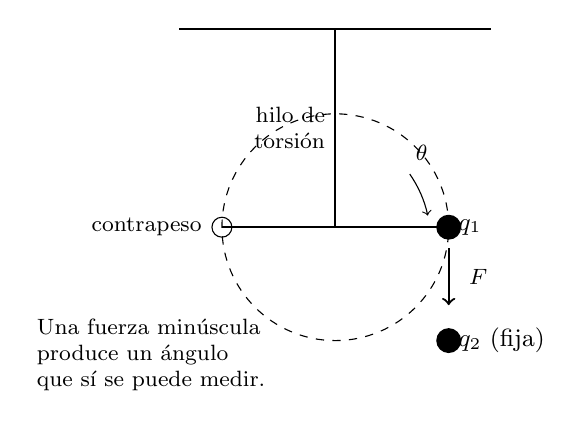
\begin{tikzpicture}[scale=0.9, every node/.style={font=\small}]
  \draw[thick] (-2.2,4) -- (2.2,4);
  \draw[thick] (0,4) -- (0,1.2) node[midway, left, font=\footnotesize, align=right]
    {hilo de\\ torsión};
  \draw[thick] (-1.6,1.2) -- (1.6,1.2);
  \fill (1.6,1.2) circle (5pt) node[right] {$q_1$};
  \draw (-1.6,1.2) circle (4pt);
  \node[left, font=\footnotesize] at (-1.75,1.2) {contrapeso};
  \fill (1.6,-0.4) circle (5pt) node[right] {$q_2$ (fija)};
  \draw[->, thick] (1.6,0.9) -- (1.6,0.1);
  \node[right, font=\footnotesize] at (1.75,0.5) {$F$};
  \draw[dashed] (0,1.2) circle (1.6);
  \draw[->] (1.05,1.95) arc (35:12:1.6);
  \node[above right, font=\footnotesize] at (1.0,2.0) {$\theta$};
  \node[align=left, font=\footnotesize] at (-2.6,-0.6)
    {Una fuerza minúscula\\ produce un ángulo\\ que sí se puede medir.};
\end{tikzpicture}
\end{center}

\begin{nota}
\textbf{Dónde suele trabarse.} En las unidades, no en la física. Vale la pena imponer una
rutina y exigirla en el quiz: (1) pasar todas las cargas a coulombs, (2) pasar la distancia a
metros, (3) reemplazar, (4) revisar que el exponente del resultado tenga sentido. La mayoría
de los errores mueren en el paso 2.
\end{nota}

\begin{nota}
\textbf{Sobre el signo.} En los ejercicios de este nivel conviene trabajar con los
\emph{valores absolutos} de las cargas para hallar la magnitud, y decidir aparte si es
atracción o repulsión mirando los signos. Meter los signos dentro de la fórmula lleva a
discusiones sobre el sentido del vector que no aportan todavía.
\end{nota}

\end{document}
